\documentclass{article}
\usepackage{graphicx}
\usepackage[utf8]{inputenc}
\usepackage[T1]{fontenc}
\usepackage[polish]{babel}  % Add Polish language support
\usepackage{hyperref} % Add this package
\usepackage{longtable} % For tables
\usepackage{booktabs}  % For tables
\usepackage{array}     % For tables
\usepackage{amsmath}
\usepackage{algpseudocode}
\usepackage{float}

\title{Teoria Współbieżności \\ Zadanie Domowe \\ Współbieżna eliminacja Gaussa}
\author{Robert Mesek}
\date{}

\begin{document}

\maketitle
\tableofcontents

\newpage

\section{Wstęp}
Zadanie polega na wykonaniu następujących etapów (dla macierzy o rozmiarze $N \times N$):
\begin{enumerate}
    \item Zlokalizowanie niepodzielnych czynności wykonywanych przez algorytm,
          nazwanie ich oraz zbudowanie alfabetu w sensie teorii śladów.
    \item Skonstruowanie relacji zależności dla alfabetu, opisującego algorytm eliminacji Gaussa.
    \item Przedstawienie algorytmu eliminacji Gaussa w postaci ciągu symboli alfabetu.
    \item Wygenerowanie grafu zależności Diekerta.
    \item Przekształcenie ciągu symboli opisującego algorytm do postaci normalnej Foaty.
\end{enumerate}

\subsection{Przykład dla macierzy $3 \times 3$}
\begin{equation}
    A x = b
\end{equation}

\begin{equation}
    \begin{bmatrix}
        2 & 1 & 3  \\
        4 & 3 & 8  \\
        6 & 5 & 16
    \end{bmatrix}
    \begin{bmatrix}
        x_1 \\
        x_2 \\
        x_3
    \end{bmatrix}
    =
    \begin{bmatrix}
        6  \\
        15 \\
        27
    \end{bmatrix}
\end{equation}

Do macierzy $A$ dodajemy wektor wyrazów wolnych $b$ jako ostatnią kolumnę:
\begin{equation}
    \left[\begin{array}{@{}ccc|c@{}}
        2 & 1 & 3 & 6 \\
        4 & 3 & 8 & 15 \\
        6 & 5 & 16 & 27
    \end{array}\right]
\end{equation}


\begin{equation}
    \left[\begin{array}{@{}ccc|c@{}}
        2 & 1 & 3 & 6 \\
        4 & 3 & 8 & 15 \\
        6 & 5 & 16 & 27
    \end{array}\right]
    \xrightarrow{\begin{array}{l} 
        w_2 \mathrel{-}= 2w_1 \\
        w_3 \mathrel{-}= 3w_1
    \end{array}}
    \left[\begin{array}{@{}ccc|c@{}}
        2 & 1 & 3 & 6 \\
        0 & 1 & 2 & 3 \\
        0 & 2 & 7 & 9
    \end{array}\right]
\end{equation}
\begin{equation}
    \left[\begin{array}{@{}ccc|c@{}}
        2 & 1 & 3 & 6 \\
        0 & 1 & 2 & 3 \\
        0 & 2 & 7 & 9
    \end{array}\right]
    \xrightarrow{\begin{array}{l} 
        w_3 \mathrel{-}= 2w_2
    \end{array}}
    \left[\begin{array}{@{}ccc|c@{}}
        2 & 1 & 3 & 6 \\
        0 & 1 & 2 & 3 \\
        0 & 0 & 3 & 3
    \end{array}\right]
\end{equation}

Pozostaje nam rozwiązać układ równań wykonując podstawienia wsteczne:
\begin{equation}
    \left[\begin{array}{@{}ccc|c@{}}
        2 & 1 & 3 & 6 \\
        0 & 1 & 2 & 3 \\
        0 & 0 & 3 & 3
    \end{array}\right]
    \rightarrow
    \left[\begin{array}{@{}ccc|c@{}}
        1 & 0 & 0 & 1 \\
        0 & 1 & 0 & 1 \\
        0 & 0 & 1 & 1
    \end{array}\right]
\end{equation}

Rozwiązaniem jest $x = [1, 1, 1]$

\newpage

\section{Niepodzielne czynności eliminacji Gaussa oraz alfabet}
Współbieżny algorytm eliminacji Gaussa możemy rozbić na 3 podstawowe zadania.
\subsection{Niepodzielne czynności}
% # Indivisible tasks:
% #   A_i_k: m[k, i] = M[k, i] / M[i, i]
% #          (find the multiplier for subtracting i-th row from k-th row)
% #   B_i_j_k: n[k, i, j] = M[i, j] * m[k, i]
% #            (find the product of multiplier and i-th row element)
% #   C_i_j_k: M[k, j] = M[k, j] - n[k, i, j]
% #            (subtract the product from k-th row)
% # Foata normal form:
% #   FNF_N = [A_0_k][B_0_j_k][C_0_j_k]...[A_N-1_k][B_N-1_j_k][C_N-1_j_k]
$\mathbf{i}$ - numer wiersza, który redukujemy \\
$\mathbf{j}$ - numer elementu w wierszu \\
$\mathbf{k}$ - numer wiersza, od którego odejmujemy \\
$\mathbf{M}$ - macierz z dołączonym wektorem wyrazów wolnych \\
$\mathbf{m}$ - mnożniki \\
$\mathbf{n}$ - iloczyny mnożników i elementów wiersza 
\begin{enumerate}
    \item \textbf{Zadanie $\mathbf{A_{i,k}}$}: Znalezienie mnożnika (\verb|m|) dla odejmowania i-tego wiersza od k-tego wiersza 
    (\verb|A_i_k: m[k, i] = M[k, i] / M[i, i]|)
    \item \textbf{Zadanie $\mathbf{B_{i,j,k}}$}: Znalezienie iloczynu (\verb|n|) mnożnika i elementu i-tego wiersza 
    (\verb|B_i_j_k: n[k, i, j] = M[i, j] * m[k, i]|)
    \item \textbf{Zadanie $\mathbf{C_{i,j,k}}$}: Odejmowanie iloczynu od k-tego wiersza \\
    (\verb|C_i_j_k: M[k, j] = M[k, j] - n[k, i, j]|)
\end{enumerate}

\subsection{Alfabet}
W tym przypadku alfabet będzie składał się z naszych niepodzielnych czynności, 
dla indeksów $i, j, k$ mających sens, to znaczy:
\begin{multline}
    \Sigma = \{A_{i,k}, B_{i,j,k}, C_{i,j,k} \\
    \mid i \in \{0, \ldots, N-1\}, j \in \{i, \ldots, N+1\}, k \in \{i+1, \ldots, N\}\}
\end{multline}


\section{Relacja zależności dla alfabetu}
Zależności miedzy naszymi czynnościami jesteśmy w stanie wywnioskować analizując
sposób działania algorytmu eliminacji Gaussa.

Łatwo zauważyć, że zadanie $\mathbf{A_{i,k}}$ musi zostać wykonane przed zadaniem $\mathbf{B_{i,j,k}}$,
które z kolei musi zostać wykonane przed zadaniem $\mathbf{C_{i,j,k}}$, co wynika z potrzeby 
wypełnienia mnożników (\verb|m|) oraz iloczynów (\verb|n|) przed ich użyciem.

Kolejno zauważamy, że zadanie $\mathbf{A_{i,k}}$ (czyli $\mathbf{C_{i,j,k}}$) musi zostać wykonane przed 
zadaniem $\mathbf{A_{i+1,k}}$, ponieważ modifikujemy wiersze od góry do dołu.

\mbox{}\newline
Z powyższych obserwacji relacja zależności dla $\Sigma$ będzie miała postać:
\begin{multline}
    D = \{(A_{i,k}, B_{i,j,k}), (B_{i,j,k}, C_{i,j,k}), (C_{i,j,k}, A_{i+1,k}) \\
    \mid i \in \{0, \ldots, N-1\}, j \in \{i, \ldots, N+1\}, k \in \{i+1, \ldots, N\}\}
\end{multline}

\newpage

\section{Algorytm eliminacji Gaussa w postaci ciągu symboli alfabetu} \label{sec:pseudocode}
Budowanie ciągu symboli alfabetu można przedstawić jako pseudokod, gdzie 
czynności (\textbf{Task}) oznaczają kolejne elementy ciągu:
\begin{algorithmic}[1]
    \For{$i \gets 0$ to $N-1$}
        \For{$k \gets i+1$ to $N$} \Comment{Niezależne czynności}
            \State \textbf{Task} $\mathbf{A_{i,k}}$
        \EndFor
        \For{$j \gets i$ to $N+1$} \Comment{Niezależne czynności}
            \For{$k \gets i+1$ to $N$}
                \State \textbf{Task} $\mathbf{B_{i,j,k}}$
            \EndFor
        \EndFor
        \For{$j \gets i$ to $N+1$} \Comment{Niezależne czynności}
            \For{$k \gets i+1$ to $N$}
                \State \textbf{Task} $\mathbf{C_{i,j,k}}$
            \EndFor
        \EndFor
    \EndFor
\end{algorithmic}

\newpage

\section{Graf zależności Diekerta}
Przykładowy graf zależności Diekerta dla macierzy $3 \times 3$:
\begin{figure}[H]
    \centering
    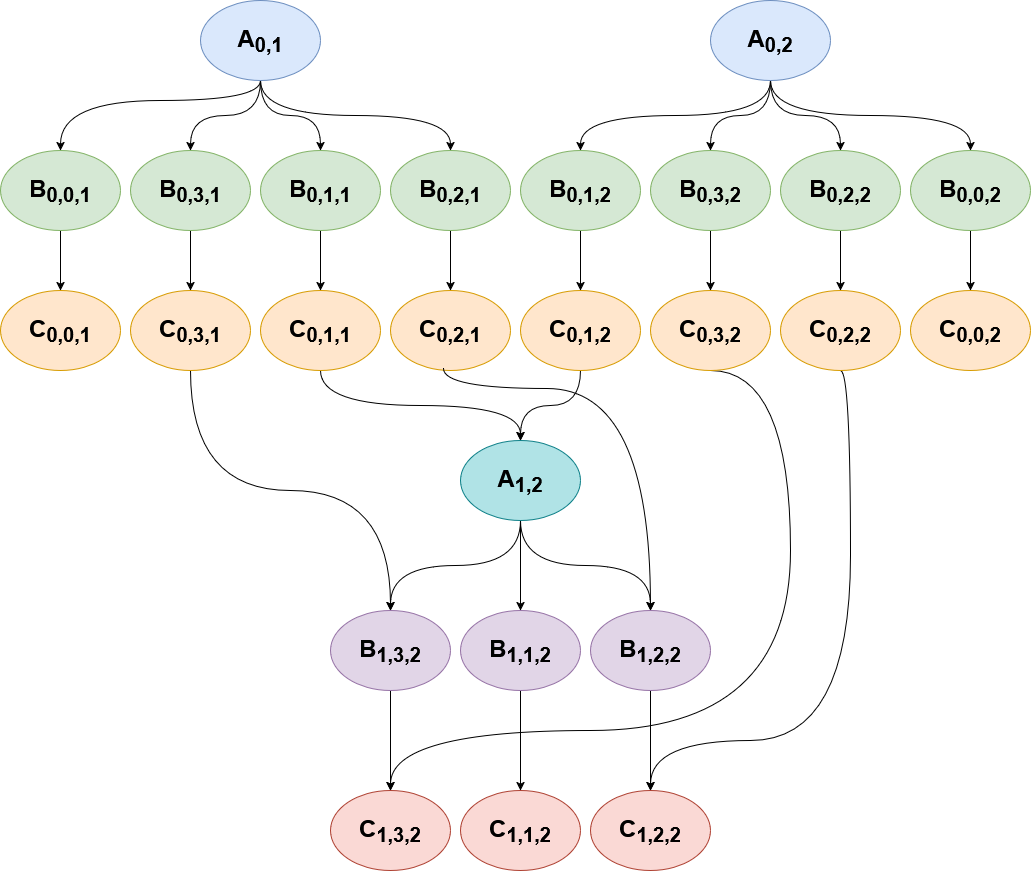
\includegraphics[width=0.8\textwidth]{images/diekert.png}
    \caption{Graf zależności Diekerta dla macierzy $3 \times 3$}
\end{figure}

\section{Przekształcenie ciągu symboli do postaci normalnej Foaty}
Przekształcenie ciągu symboli do postaci normalnej Foaty polega na zgrupowaniu 
niezależnych czynności. W tym przypadku niezależnymi klasami będą zadania z 
wewnętrznych pętli \verb|for| pseudokodu z sekcji \ref{sec:pseudocode} oznaczone komentarzami.
\begin{multline}
    \text{FNF}_N = \{[A_{i,k} \mid k \in \{i+1, \ldots, N\}] \\
    [B_{i,j,k} \mid j \in \{i, \ldots, N+1\}, k \in \{i+1, \ldots, N\}] \\
    [C_{i,j,k} \mid j \in \{i, \ldots, N+1\}, k \in \{i+1, \ldots, N\}] \\
    \mid i \in \{0, \ldots, N-1\}\}
\end{multline}

\newpage

\section{Program w języku Python}
Implementacja współbieżnej eliminacja Gaussa została zrealizowana w języku Python
z wykorzystaniem biblioteki \verb|NumPy|.

\subsection{Uruchomienie programu}
\begin{verbatim}
python main.py [-h] -i INPUT -o OUTPUT
\end{verbatim}
Program został przetestowany pod kontrolą systemu operacyjnego \verb|Ubuntu 24|
dla wersji
\begin{itemize}
    \item \verb|Python 3.12.7| z \verb|NumPy 2.1.3|
    \item \verb|Python 3.13.1t| z \verb|NumPy 2.2.0|
\end{itemize}


\end{document}